\section{Statistiques descriptives bivariées sur des données d’Iris}
\subsection{Étude de la largeur du pétale en fonction de la longueur du pétale}
\subsubsection*{Représentation graphique}
\vspace{.2cm}

%%%%%
\noindent
\textbf{Question~1~:} Tracer le nuage de points de la longueur du pétale en fonction de la largeur du pétale
pour les 150 iris contenus dans les données ((numpy.)plot, (numpy.)scatter). Ne pas oublier de
mettre des titres sur les axes. Décrire le nuage de points.
\vspace{.2cm}


\begin{figure}[!h]
    \centering
    \begin{minipage}{.60\linewidth}
        \begin{center}
            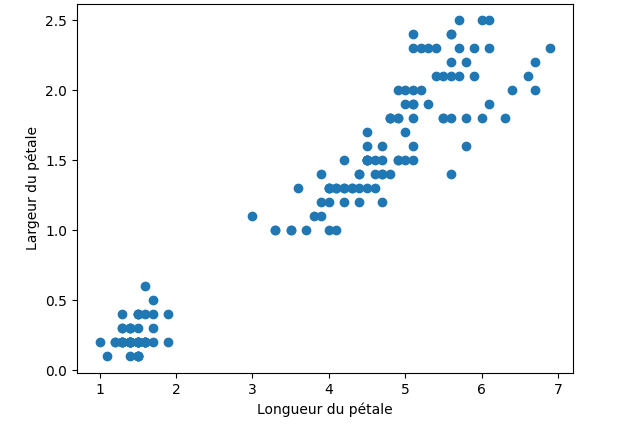
\includegraphics[width=1\textwidth]{img/Figure_1.png}
            \caption{\label{fig:figure1}Nuage de points de la longueur en fonction de la largeur du pétale des 150 Iris}
        \end{center}
    \end{minipage}\hfill
    \begin{minipage}{.36\linewidth}
        Dans un premier temps, on remarque deux concentrations principale. \\
        La première a une longueur de pétale qui varie entre 1~cm et 2~cm pour une largeur d’environ 0,2~cm et 0,6~cm. La seconde, une longueur variant de 3~cm à 7~cm avec une largeur de 
        1~cm à 2,5~cm. \\

        \noindent
        On constate également que la longueur de pétale varie proportionnellement à la largeur.
    \end{minipage}
\end{figure}

\begin{lstlisting}[style=myPython, caption=Code Python pour calculer le coefficient de corrélation, frame=lines]
plt.scatter(petallength, petalwidth)
plt.ylabel("Largeur du pétale")
plt.xlabel("Longueur du pétale")
plt.title("Nuage de points de la longueur en fonction de la largeur du pétale")
plt.show()
\end{lstlisting}

\clearpage

%%%%%
\noindent
\textbf{Question~2~:} Rappeler la définition du coefficient de corrélation et le calculer par la fonction ((numpy.)corrcoef)
\vspace{.2cm}

Le coefficient de corrélation est une valeur qui permet de déterminer s'il existe une relation linéaire entre deux variables, ce qui veut dire que si ces variables sont corrélées alors elles sont liées. \\


\begin{lstlisting}[style=myPython, caption=Code Python pour calculer le coefficient de corrélation, frame=lines]
corr_coef_matrix = np.corrcoef(petallength, petalwidth)
print("Matrice de corrélation:\n",corr_coef_matrix)
\end{lstlisting}

\begin{lstlisting}[style=myLog, caption=Résultat du code, frame=lines]
Matrice de corrélation:
[[1.        0.9627571]
[0.9627571 1.       ]]
\end{lstlisting}

\vspace{.5cm}


%%%%%
\noindent
\textbf{Question~3~:} Donner l’équation de la droite de régression linéaire, créer une fonction permettant de la
calculer à partir de deux variables X et Y et tracer la sur le même graphique
\vspace{.2cm}

\begin{enumerate}
    \item \textbf{Résultat et analyse~:}
        \begin{figure}[!h]
            \centering
            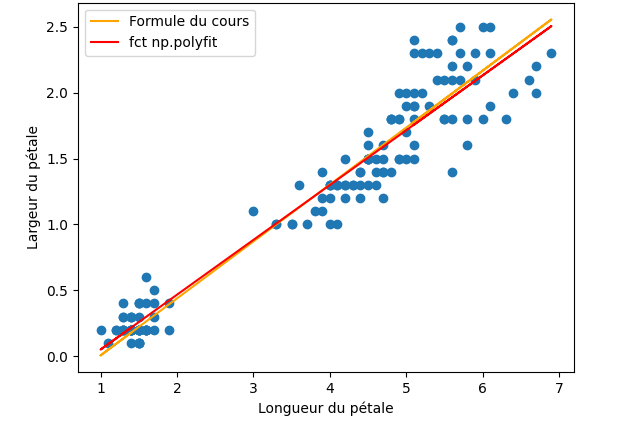
\includegraphics[width=.6\textwidth]{img/Figure_2.png}
            \caption{\label{fig:figure2}Équation de la droite de régression linéaire sur le nuage de points}
        \end{figure}

    \item \textbf{Formules utilisées~:}
        \begin{gather}
            \hat{a} = \rho_{X,Y}.\frac{S_{n-1,Y}}{S_{n-1,X}} \qquad \text{et} \qquad \hat{b} = \overline{Y_{n}}.\rho_{X,Y}.\frac{S_{n-1,Y}}{S_{n-1,X}}.\overline{X_{n}}
        \end{gather}

        \vspace{.5cm}

    \item \textbf{Code python~:}
        \begin{lstlisting}[style=myPython, caption=Code Python pour tracer la droite de régression linéaire, frame=lines]
# Méthode par la formule du cours
def regression_lineaire(corr_coef, x, y):
    mean_x = np.mean(x)
    var_x = np.var(x)
    e_type_x = np.sqrt(var_x)

    mean_y = np.mean(y)
    var_y = np.var(y)
    e_type_y = np.sqrt(var_y)

    a = corr_coef * (e_type_y/e_type_x)
    b = mean_y - corr_coef * ((e_type_y/e_type_x)) * mean_x

    return a, b


a, b = regression_lineaire(corr_coef, petallength, petalwidth)

# Méthode avec polyfit de numpy
fit = np.polyfit(petallength, petalwidth, 1)
poly = petallength*fit[0]+fit[1]

plt.plot(petallength, a*petallength+b, color='orange', label='Formule du cours')
plt.plot(petallength, poly, color='red', label='fct np.polyfit')
plt.scatter(petallength, petalwidth)
plt.ylabel("Largeur du pétale")
plt.xlabel("Longueur du pétale")
plt.title("Equation de la droite de régression linéaire")
plt.legend()
plt.show()
        \end{lstlisting}
    
    \vspace{.2cm}
\end{enumerate}









\vspace{.5cm}


%%%%%
\noindent
\textbf{Question~4~:} Analyser le lien entre les deux variables
\vspace{.2cm}

On constate que les variables \textit{petalLenght} et \textit{petalWidth} sont liées, elles évoluent proportionnellement l'une avec l'autre. \\
On peut donc soumettre l'hypothèse que ces variables sont corrélées puisqu'il existe deux réels tels que $Y=aX+b$.

\vspace{.3cm}
